\chapter{Синхронизација календара за \textit{оwnCloud} платформу}
\label{chap:ownCloudCalendarSynchronization}

У претходним поглављима описани су основни концепти технологија и окружења који су коришћени у развоју датог пројекта, са циљем да се читаоцу омогући да формира слику комплетног, заокруженог, решења. Сам пројекат, који је тема овог рада, може се посматрати као део тог решења. У овом поглављу фокус ће бити постављен на појашњења неких делова његове имплементације.

\section{Жељене функционалности}

Актуелна, званична, верзија \textit{оwnCloud} десктоп клијента обезбеђује само синхронизацију докумената који се налазе на \textit{оwnCloud} платформи. Основни циљ овог пројекта јесте да се развије решење, у виду мултиплатформског десктоп клијента, које би омогућило преузимање информација о креираним догађајима на \textit{оwnCloud} календару и приказ одговарајућих обавештења. Апликација има следећи скуп функционалности:
\begin{enumerate}
	\item синхронизација догађаја на захтев,
	\item аутоматска синхронизација догађаја,
	\item могућност управљања аутоматском синхронизацијом (потребна/није потребна, дефинисање временског интервала након којег ће се стартовати,...),
	\item приступ делу за администрацију догађаја на веб порталу \textit{оwnCloud} платформе,
	\item приказ одговарајућег обавештења, непосредно пре почетка неког догађаја,
	\item преглед преузетих догађаја.
\end{enumerate}

Ток активности које треба да обезбеде ове функционалности описан је на дијаграму \ref{fig:application_alogorithm}.

\begin{figure}[H]
	\centering
	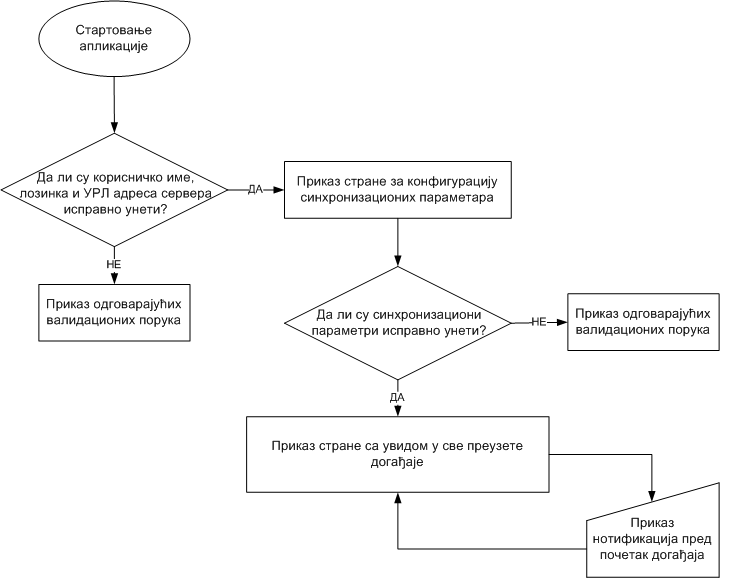
\includegraphics[scale=0.5]{slike/tok_aktivnosti.png}
	\caption{Дијаграм тока активности}
	\label{fig:application_alogorithm}
\end{figure}

На основу приказаног алгоритма  може се стећи јасна и потпуна слика о начину рада саме апликације. У наставку ће бити детаљније објашњене неке интересантније функционалности и биће приказани делови програмског кода, док се комплетан код пројекта може погледати на одговарајућем репозиторијуму\cite{svn_repo}.